% A LaTeX template for EXECUTIVE SUMMARY of the MSc Thesis submissions to
% Politecnico di Milano (PoliMi) - School of Industrial and Information Engineering
%
% S. Bonetti, A. Gruttadauria, G. Mescolini, A. Zingaro
% e-mail: template-tesi-ingind@polimi.it
%
% Last Revision: October 2021
%
% Copyright 2021 Politecnico di Milano, Italy. NC-BY

\documentclass[11pt,a4paper,twocolumn]{article}

%------------------------------------------------------------------------------
%	REQUIRED PACKAGES AND  CONFIGURATIONS
%------------------------------------------------------------------------------
% PACKAGES FOR TITLES
\usepackage{titlesec}
\usepackage{color}

% PACKAGES FOR LANGUAGE AND FONT
\usepackage[utf8]{inputenc}
\usepackage[english]{babel}
\usepackage[T1]{fontenc} % Font encoding

% PACKAGES FOR IMAGES
\usepackage{graphicx}
\graphicspath{{Images/}} % Path for images' folder
\usepackage{eso-pic} % For the background picture on the title page
\usepackage{subfig} % Numbered and caption subfigures using \subfloat
\usepackage{caption} % Coloured captions
\usepackage{transparent}

% STANDARD MATH PACKAGES
\usepackage{amsmath}
\usepackage{amsthm}
\usepackage{bm}
\usepackage[overload]{empheq}  % For braced-style systems of equations

% PACKAGES FOR TABLES
\usepackage{tabularx}
\usepackage{longtable} % tables that can span several pages
\usepackage{colortbl}

% PACKAGES FOR ALGORITHMS (PSEUDO-CODE)
\usepackage{algorithm}
\usepackage{algorithmic}

% PACKAGES FOR REFERENCES & BIBLIOGRAPHY
\usepackage[colorlinks=true,linkcolor=black,anchorcolor=black,citecolor=black,filecolor=black,menucolor=black,runcolor=black,urlcolor=black]{hyperref} % Adds clickable links at references
\usepackage{cleveref}
\usepackage[square, numbers, sort&compress]{natbib} % Square brackets, citing references with numbers, citations sorted by appearance in the text and compressed
\bibliographystyle{unsrt} % Same style as the thesis: references ordered by citation appearance

% PACKAGES FOR THE APPENDIX
\usepackage{appendix}

% PACKAGES FOR ITEMIZE & ENUMERATES
\usepackage{enumitem}

% OTHER PACKAGES
\usepackage{amsthm,thmtools,xcolor} % Coloured "Theorem"
\usepackage{comment} % Comment part of code
\usepackage{fancyhdr} % Fancy headers and footers
\usepackage{lipsum} % Insert dummy text
\usepackage{tcolorbox} % Create coloured boxes (e.g. the one for the key-words)
\usepackage{stfloats} % Correct position of the tables

%-------------------------------------------------------------------------
%	NEW COMMANDS DEFINED
%-------------------------------------------------------------------------
% EXAMPLES OF NEW COMMANDS -> here you see how to define new commands
\newcommand{\bea}{\begin{eqnarray}} % Shortcut for equation arrays
\newcommand{\eea}{\end{eqnarray}}
\newcommand{\e}[1]{\times 10^{#1}}  % Powers of 10 notation
\newcommand{\mathbbm}[1]{\text{\usefont{U}{bbm}{m}{n}#1}} % From mathbbm.sty
\newcommand{\pdev}[2]{\frac{\partial#1}{\partial#2}}
% NB: you can also override some existing commands with the keyword \renewcommand

%----------------------------------------------------------------------------
%	ADD YOUR PACKAGES (be careful of package interaction)
%----------------------------------------------------------------------------


%----------------------------------------------------------------------------
%	ADD YOUR DEFINITIONS AND COMMANDS (be careful of existing commands)
%----------------------------------------------------------------------------


% Do not change Configuration_files/config.tex file unless you really know what you are doing.
% This file ends the configuration procedures (e.g. customizing commands, definition of new commands)
\input{Configuration_files/config}

% Insert here the info that will be displayed into your Title page
% -> title of your work
\renewcommand{\title}{Profiling Framework for LLM-Based Data Agents: Quality, Latency, and Energy under Parameter Sensitivity}
% -> author name and surname
\renewcommand{\author}{Davide Valenzisi}
% -> author student ID (matricola)
\newcommand{\ID}{245001}
% -> second author name and surname (if any, otherwise leave empty)
\newcommand{\secondauthor}{Ossama El Oukili}
% -> second author student ID (if any, otherwise leave empty)
\newcommand{\secondID}{996171}
% -> MSc course
\newcommand{\course}{Computer Science and Engineering - Ingegneria Informatica}
% -> advisor name and surname
\newcommand{\advisor}{Prof. Danilo Ardagna}
% IF AND ONLY IF you need to modify the co-supervisors you also have to modify the file Configuration_files/title_page_summary.tex (ONLY where it is marked)
%\newcommand{\firstcoadvisor}{Name Surname} % insert if any otherwise comment
%\newcommand{\secondcoadvisor}{Name Surname} % insert if any otherwise comment
% -> academic year
\newcommand{\YEAR}{2025-2026}
% -> abstract shown in the title page
\renewcommand{\abstract}{Large Language Models (LLMs) increasingly power natural language
interfaces to structured data, yet deploying them in production raises concerns beyond
accuracy, namely inference latency and energy cost. To study these concerns, this work builds
a \textit{Sales Agent}: an LLM-powered system, orchestrated with LangGraph, that translates a
business question into a SQL query executed over Parquet files via DuckDB, interprets the
results in text, and optionally renders a chart. A hierarchical YAML configuration exposes the
inference parameters studied in the experiments (sampling parameters, best-of-$N$, token budgets,
and Chain-of-Thought refinement depth) across open-weight models served locally via Ollama. The
core contribution is a systematic profiling that jointly measures output quality, execution time,
and per-step energy consumption (via CodeCarbon), over 20 analytical questions stratified across
four SQL difficulty levels. Five step-isolated experiments establish a baseline for three
open-weight models and then vary one agent step at a time. The experiments also challenge the
assumption that larger thinking models are always the best solution. The results show instead
that model choice alone does not explain performance: the dominant effects arise from the interaction between model
family, agent step, prompt difficulty, and inference-time settings. The thesis distills three
recommendations for energy-aware LLM data agents: tune hyperparameters per agent step rather than
globally, allocate inference-time compute by failure mode, and report accuracy and energy by
prompt difficulty.}
% -> key-words shown in the coloured box of the title page
\newcommand{\keywords}{LLM data agents, Energy-aware profiling, Quality-energy trade-off, Local open-weight LLMs, LLM-as-judge evaluation}

%-------------------------------------------------------------------------
%	BEGIN OF YOUR DOCUMENT
%-------------------------------------------------------------------------
\begin{document}

%-----------------------------------------------------------------------------
% TITLE PAGE
%-----------------------------------------------------------------------------
% Do not change Configuration_files/TitlePage.tex (Modify it IF AND ONLY IF you need to add or delete the Co-advisors)
% This file creates the Title Page of the document.
% NB: the Executive Summary uses its OWN title page (title_page_summary),
% NOT the thesis one (Configuration_files/title_page).
% The file already provides its own \twocolumn[{...}] wrapper, so DO NOT wrap it again.
\input{Configuration_files/title_page_summary}

%%%%%%%%%%%%%%%%%%%%%%%%%%%%%%
%%     THESIS MAIN TEXT     %%
%%%%%%%%%%%%%%%%%%%%%%%%%%%%%%

%-----------------------------------------------------------------------------
% INTRODUCTION
%-----------------------------------------------------------------------------
\section{Introduction}
\label{sec:introduction}

The growing adoption of Large Language Models (LLMs) in enterprise software has opened a concrete
path toward natural language interfaces for structured data. A system that translates a business
question into a SQL query, executes it, and returns both a textual analysis and a chart makes
data-driven decision making accessible to non-technical users. Deploying such systems in
production, however, raises practical questions that go beyond accuracy: how long does each
inference take, how does it scale with configuration changes, and what is the energy cost of
running LLM-backed pipelines on real hardware? These efficiency concerns are central to
sustainable AI~\cite{strubell2019energy, schwartz2020greenai}, yet they are rarely measured
jointly with quality for LLM-based data agents.

This work addresses both sides of the problem. On the application side, it presents the design
and implementation of a \textit{Sales Agent}: an LLM-powered conversational system that lets a
business analyst query a synthetic retail dataset in plain English. Given a natural language
question, the agent autonomously selects the processing steps, generates and executes a SQL query
against Parquet files via DuckDB, produces a textual interpretation of the results, and optionally
renders a Matplotlib chart. The agent is orchestrated through LangGraph~\cite{langgraph}, a
framework for stateful graph-based LLM pipelines, and runs on locally-hosted open-weight models
served via Ollama. A hierarchical YAML configuration exposes the inference parameters studied in the experiments ---
sampling temperature, top-$p$, top-$k$, best-of-$N$ candidates, and Chain-of-Thought
refinement depth --- making each run fully reproducible and configurable
without code changes.

On the experimental side, the core contribution is the systematic \emph{profiling} of the agent,
which jointly measures output quality, execution time, and per-step energy consumption (tracked
with CodeCarbon~\cite{lottick2019codecarbon}). A benchmark of 20 analytical questions, stratified
across four SQL difficulty levels, evaluates quality along three complementary dimensions: a
graded ground-truth table-similarity score for data retrieval, and two LLM-as-judge
scores~\cite{zheng2023judging} for the textual analysis and the visualization. The evaluation is
organised as five step-isolated experiments: the first establishes a quality and energy baseline
for three open-weight models (Gemma~4~E4B, Gemma~4~26B, and Mistral~Small~3.2~24B), and the
following four vary one agent step at a time across sampling hyperparameters, token budgets, and
inference-time compute, closing with a Pareto confirmation run. The central finding is that model
choice alone does not explain performance: the dominant effects arise from the interaction between
model family, agent step, prompt difficulty, and inference-time settings. From this analysis the
thesis distills three recommendations for energy-aware LLM data agents --- tune hyperparameters
per agent step rather than globally, allocate inference-time compute by failure mode, and report
accuracy and energy by prompt difficulty.

%-----------------------------------------------------------------------------
% THE SALES AGENT
%-----------------------------------------------------------------------------
\section{The Sales Agent}
\label{sec:es_application}

The Sales Agent lets a business analyst query a synthetic retail dataset in natural
language, without writing SQL. The dataset consists of three Parquet tables ---
\textit{sales} (daily store-level transactions), \textit{products} (catalog), and
\textit{stores} (metadata) --- linked by shared keys, so questions can span multiple
entities through SQL joins. Given a question, the agent retrieves the relevant data,
produces a textual analysis, and optionally renders a chart, returning a CSV table, a
natural language interpretation, and executable Matplotlib code.

\paragraph{Architecture.}
The agent is orchestrated as a stateful directed graph built with
LangGraph~\cite{langgraph} (Figure~\ref{fig:es_overview}). A \texttt{decide\_tool} node
acts as a router that, at each iteration, invokes the LLM to choose the next action and
loops back until termination. Three processing nodes encapsulate the analytical
capabilities: \texttt{lookup} generates a SQL query from the prompt and the database
schema and executes it via DuckDB; \texttt{analysis} interprets the retrieved data in
text; and \texttt{visualization} produces a chart configuration and the Matplotlib code,
which is validated by execution and, on failure, repaired through error-aware refinement
when CoT refinement is enabled.
A shared \texttt{State} object carries the prompt, the data, the generated SQL, the per-step
timings and scores between nodes. The LLM backbone is provider-agnostic: open-weight models
are served locally via Ollama (used for the agent), while the OpenAI API is reserved for
the LLM-as-judge evaluation.

\begin{figure}[t]
    \centering
    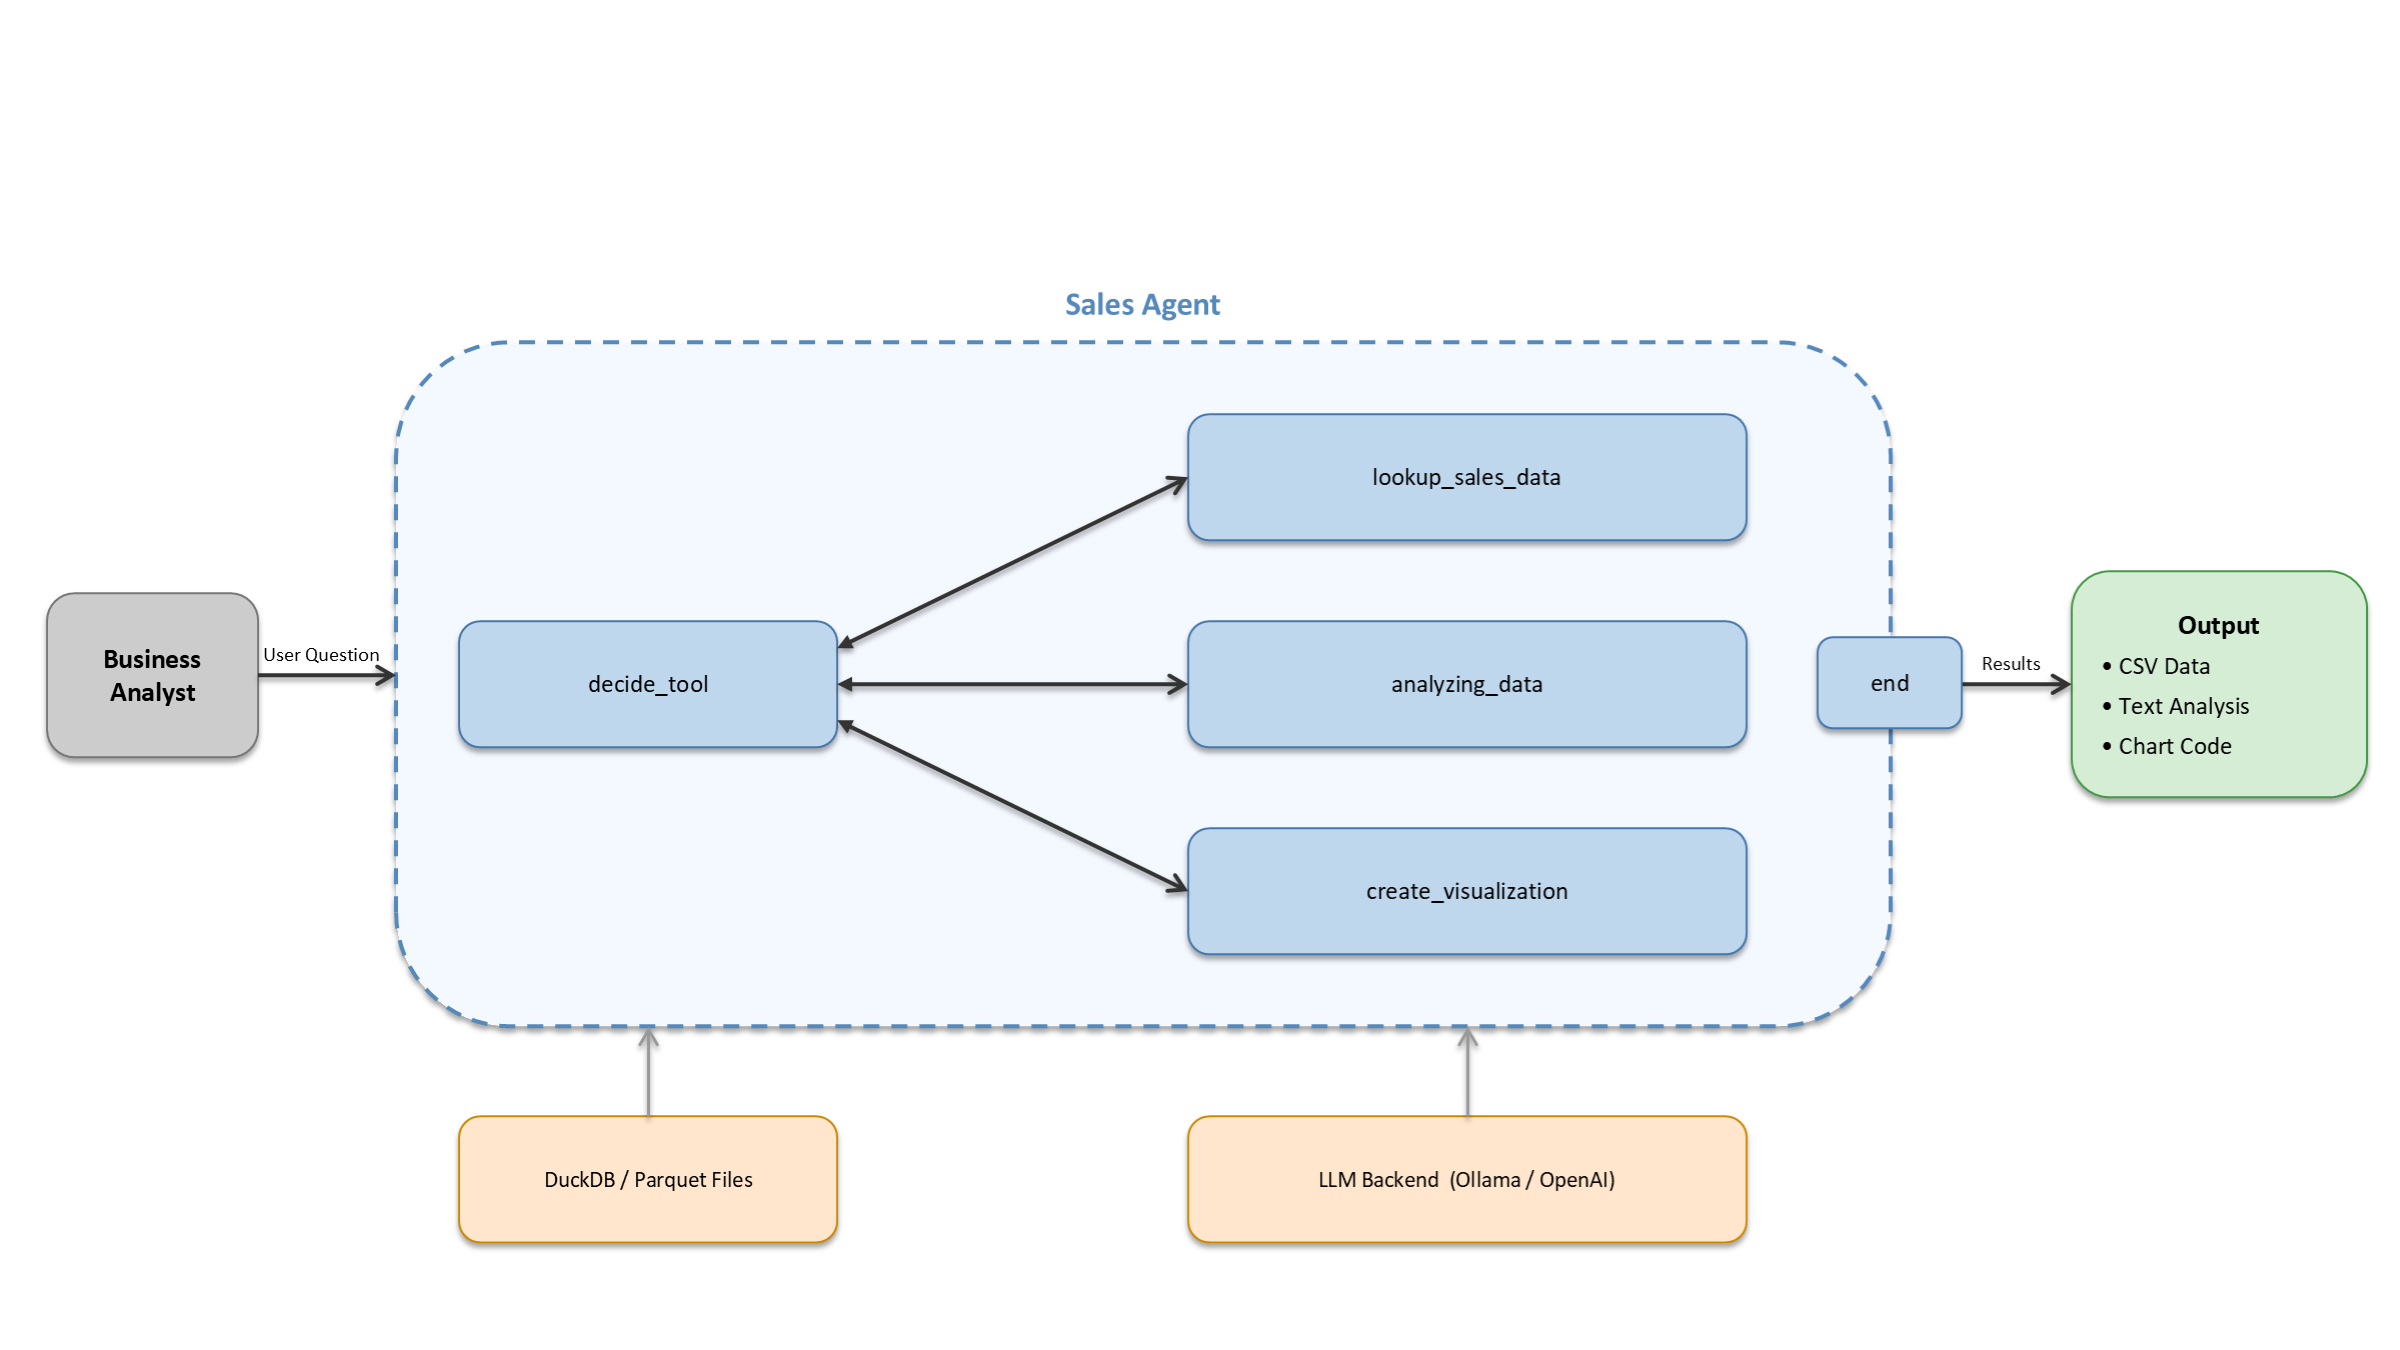
\includegraphics[width=\columnwidth]{Images/fig1_system_overview}
    \caption{High-level architecture of the Sales Agent.}
    \label{fig:es_overview}
\end{figure}

\paragraph{Configuration and inference-time mechanisms.}
A hierarchical YAML configuration exposes the inference parameters studied in the experiments
\emph{per agent step} --- sampling temperature, top-$p$, top-$k$, token budget,
best-of-$N$ candidates, and Chain-of-Thought (CoT) refinement depth --- so that each run is
fully reproducible without code changes. Two inference-time compute mechanisms are central
to the study. \emph{Best-of-$N$} sampling runs a step $N$ times while sweeping one sampling
parameter, then selects the best candidate; during live execution the lookup step uses a
ground-truth-free, self-consistency~\cite{wang2023selfconsistency} consensus evaluator that
picks the candidate with the highest average row-level agreement with the others.
\emph{Iterative CoT refinement} feeds a step's output back into the
prompt for up to a configured number of iterations, stopping early on convergence; in
error-aware mode it injects the execution error so the model can self-correct.

\paragraph{Benchmark and metrics.}
The agent is evaluated on a hand-built benchmark of 20 analytical questions, stratified
across four SQL difficulty levels (from single-table aggregations to multi-join queries
with ratios and year-over-year logic). Quality is measured per step along three
complementary dimensions: a graded table-similarity score between the
retrieved table and the ground truth for lookup; and two LLM-as-judge~\cite{zheng2023judging}
scores --- factual accuracy and coverage for the analysis, and axis/type/functional
correctness for the visualization. Energy is tracked with CodeCarbon~\cite{lottick2019codecarbon},
which records CPU, GPU, and RAM energy draw both per step and for the whole run, alongside
wall-clock latency. This makes quality, latency, and energy directly comparable across
configurations.

%-----------------------------------------------------------------------------
% EXPERIMENTAL DESIGN
%-----------------------------------------------------------------------------
\section{Experimental Design}
\label{sec:es_design}

Three open-weight models are studied, served locally via Ollama:
Gemma~4~E4B~\cite{gemma4_2025}, a compact reasoning model; Gemma~4~26B, its large
counterpart; and Mistral~Small~3.2~24B~\cite{mistralsmall_2025}, an instruction-following
model. Each model uses the sampling defaults recommended on its Ollama page (Gemma at
temperature~1.0, Mistral at~0.15). Inference is offloaded to the GPU, while
LLM-as-judge scoring uses the OpenAI API. Experiments were executed on
two GPU servers (NVIDIA~L40S and A40) to parallelise data collection: absolute latency and
energy are not compared across machines, but each sweep varies a single factor on a fixed
machine, so the rankings and relative trends it captures are unaffected.

The campaign is structured as five \emph{step-isolated} experiments, each isolating one
aspect of behaviour:

\begin{itemize}[noitemsep,topsep=2pt]
    \item \textbf{Test 01 --- Baseline.} Each model is run with its default configuration on
          the full 20-prompt benchmark, establishing a quality and energy reference.
    \item \textbf{Test 02 --- Sensitivity (OFAT).} Five static sampling hyperparameters
          (temperature, top-$p$, top-$k$, repeat penalty, repeat-window) are swept
          one-factor-at-a-time, ten values each, separately for every agent step.
    \item \textbf{Test 03 --- Token-budget ladder.} The \texttt{max\_tokens} cap is varied
          across four levels per step to find the minimum safe budget and any quality
          sensitivity to it.
    \item \textbf{Test 04 --- Compute expansion.} CoT refinement depth is swept
          ($1$--$4$) on the lookup and visualization steps; a separate follow-up (04b) instead
          studies whether \emph{best-of-$N$} sampling helps the lookup step, comparing
          best-of-$3$ temperature ranges against static temperatures (with a CoT reference).
    \item \textbf{Test 05 --- Pareto confirmation.} The most promising \emph{combined}
          per-step policies from Tests~02--04 are evaluated on the full benchmark to fix the
          definitive quality-versus-energy frontier.
\end{itemize}

Latency and energy are treated as two readings of the same cost: on fixed hardware the GPU
draws near-constant power during generation, so per-prompt energy is essentially a fixed
multiple of wall-clock time (the per-model latency and energy rankings coincide to within
about five percentage points). The trade-off analysis therefore uses \emph{energy per prompt}
as the single efficiency axis.

%-----------------------------------------------------------------------------
% RESULTS
%-----------------------------------------------------------------------------
\section{Results}
\label{sec:es_results}

\paragraph{Baseline (Test 01).}
At default settings, no model dominates: the three have distinct, \emph{step-specific}
failure modes. Mistral~Small is the Pareto baseline --- the highest strict (end-to-end)
quality, 0.827, at the lowest cost (48.9~s and 0.00601~kWh per prompt) --- but it collapses
deterministically on the two hardest difficulty-4 aggregation prompts. Gemma~E4B nearly
matches its quality (0.821) with the most balanced per-step profile, but at $1.47\times$ the
energy and $1.54\times$ the latency (0.00883~kWh, 75.4~s), and it shows the same lookup
brittleness on hard SQL. Gemma~26B has the strongest data-retrieval and analysis scores yet
is held back by a weak visualization step (0.500 against $0.77$--$0.78$ for the others) and
the highest cost (0.01667~kWh, 136.0~s), leaving it Pareto-dominated at baseline.

\paragraph{Sensitivity to sampling parameters (Test 02).}
The one-factor-at-a-time sweep is where the most informative patterns emerge, and its key
message is that sensitivity to static sampling parameters is a \emph{model-level} property,
not a step-level one. Gemma~E4B is by far the most sensitive model: its lookup quality alone
spans 0.223 points between the best and worst single setting, more than any step of the other
two models. This fragility is also a high-upside, cheap lever --- \texttt{top\_p}~$=0.94$
raises lookup quality by $+0.117$ and \texttt{csv\_iou} by $+0.139$ for only
$5\times10^{-4}$~kWh/prompt --- and it is the first concrete sign that the compact model's
weak baseline is a \emph{tuning} problem, not a capacity ceiling. Gemma~26B is also highly
tunable but asymmetric: every parameter family improves its weak visualization step (up to
$+0.068$ quality), yet a single bad \texttt{top\_k} value can collapse lookup quality by
$-0.123$, and lowering temperature below~1.0 actively hurts its analysis --- evidence that the
thinking model relies on sampling diversity. Mistral, by contrast, is essentially insensitive:
no parameter at any step moves quality by more than $+0.007$, so its efficiency is robust to
misconfiguration but offers almost no tuning upside (its one real risk is a
\texttt{repeat\_penalty}~$=1.2$ analysis setting that loses $0.099$ quality). Two
cross-cutting findings stand out: quality-improving settings barely
move energy (tuning is mostly a quality concern, not a cost one), and prompt difficulty
\emph{amplifies} tuning effects --- the largest swings concentrate on difficulty-4 prompts for
both thinking models. Figure~\ref{fig:es_test02_heatmap} summarises, per (step, parameter)
pair, the best achievable quality delta.

\begin{figure}[t]
    \centering
    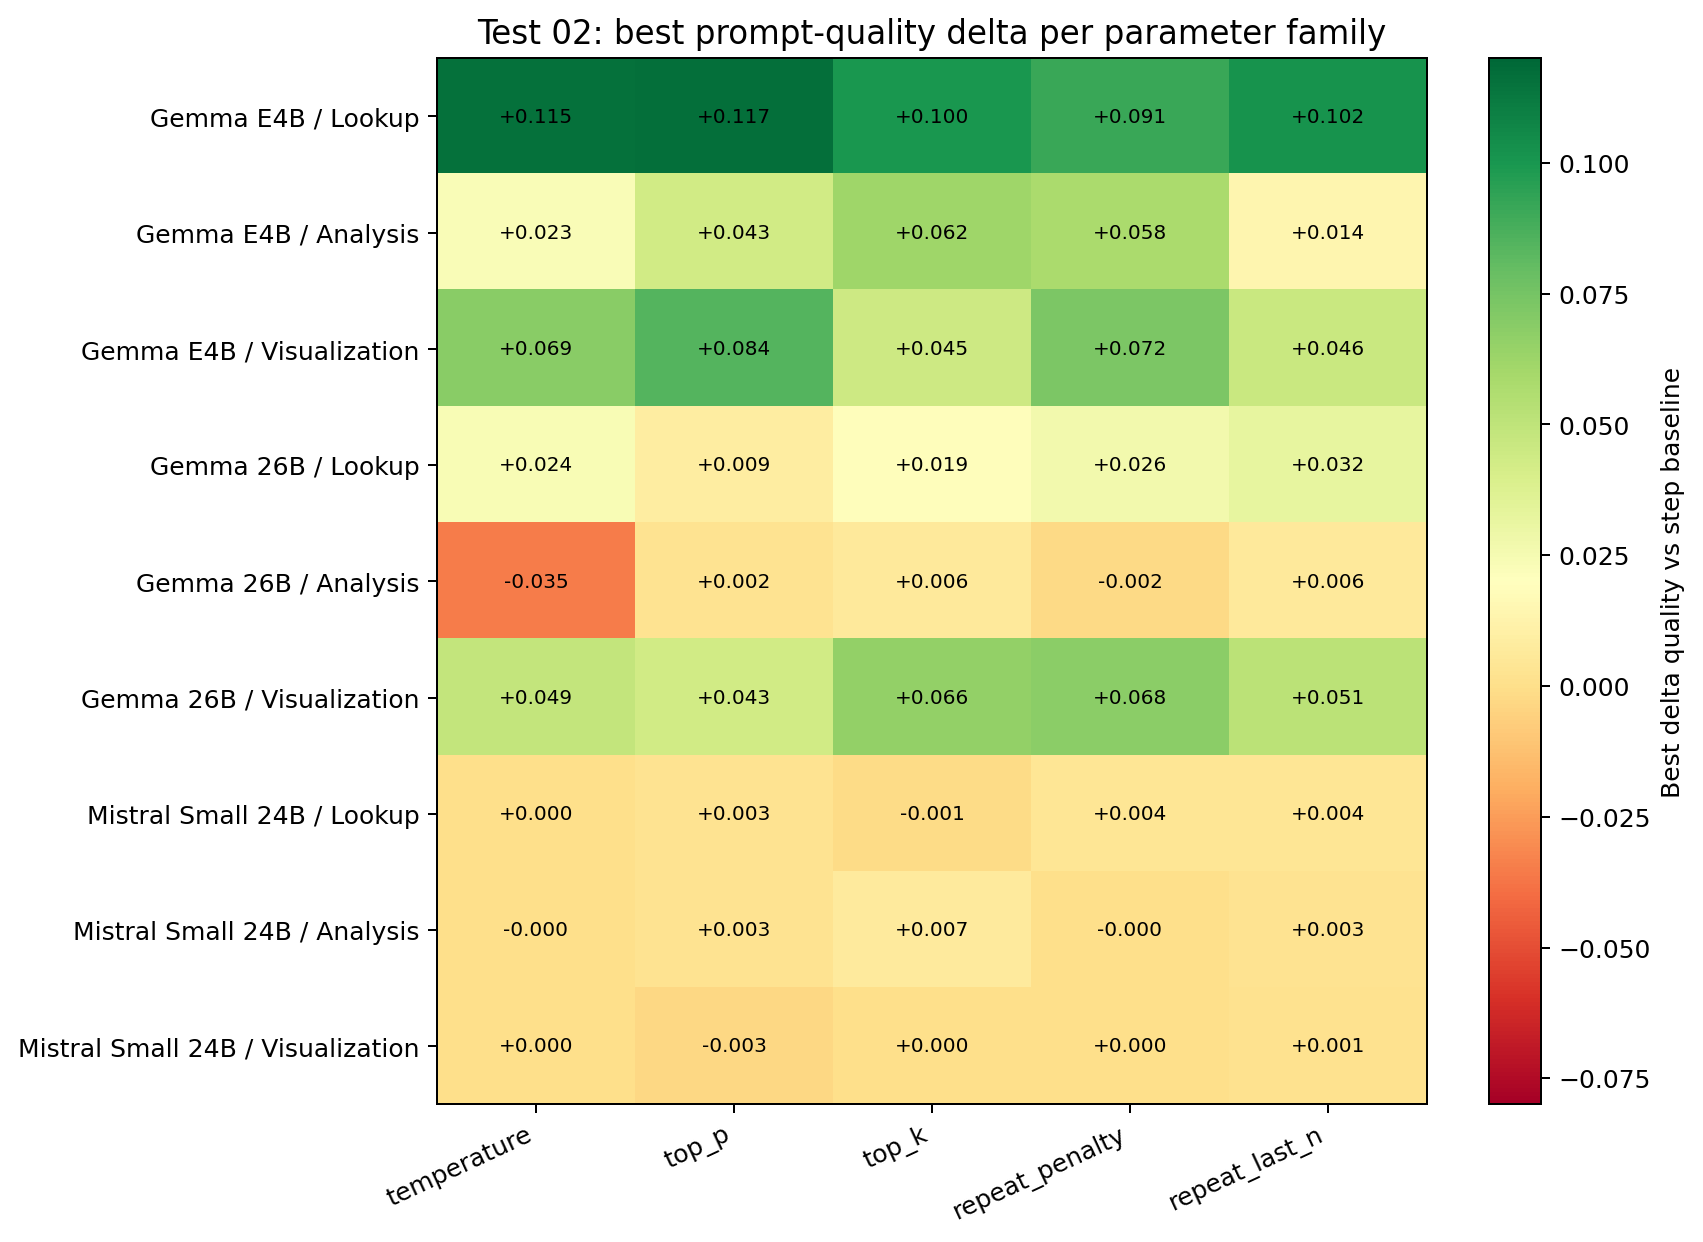
\includegraphics[width=\columnwidth]{Images/test02v2_quality_delta_heatmap.png}
    \caption{Test~02: best quality delta per (step, parameter) pair for all runs.}
    \label{fig:es_test02_heatmap}
\end{figure}

\paragraph{Token budget and inference-time compute (Tests 03--04).}
The \texttt{max\_tokens} budget (Test 03) behaves as a per-step \emph{safety bound} rather
than a quality dial: it barely affects energy, since the model stops once its output is
complete, so raising it is nearly free where a step is genuinely truncated --- Gemma~26B
visualization gains $+0.054$ \texttt{vis\_score} from a larger cap, with no plateau yet
visible within the tested range --- while overly generous caps can destabilise Gemma~E4B into
longer, worse output. The decisive lever is
\emph{inference-time compute} (Test 04): iterative CoT refinement on the lookup step lifts
Gemma~E4B by $+0.186$ quality at depth~2 (\texttt{csv\_iou} $0.757\!\to\!0.954$), repairing
exactly the SQL brittleness seen at baseline, because the SQL execution result is a feedback
signal aligned with correctness; the gain concentrates on the hardest prompts ($+0.524$ at
difficulty~4). On visualization the same mechanism is harmful at every depth, because chart
errors are semantic rather than executable, so self-criticism over-edits already-working code.
An early-stop mechanism makes the executed depth saturate near~2, so depth~2 is the efficient
default. A targeted follow-up (Test 04b) shows that best-of-$N$ temperature sampling can create
useful lookup diversity, especially with the medium range $[0.6,1.0]$, but the no-GT selector
still picks the first candidate in most runs. A well-chosen static lookup temperature is
therefore the best low-cost option, while CoT remains the stronger quality intervention.

\paragraph{Final trade-off (Test 05).}
Combining the per-step interventions yields the unified quality--energy frontier of
Figure~\ref{fig:es_pareto}. The frontier is \emph{not} a model-size ranking. Mistral with
lookup CoT defines the evaluated frontier, from the cheapest useful points around
0.0036~kWh to the highest-quality endpoint: 0.9395 prompt quality, full completion,
and 0.00453~kWh per prompt. Gemma~E4B --- repaired through lookup CoT at a lower
temperature with leaner downstream token caps --- remains extremely close
(0.9371 prompt quality at full completion), but it is slightly more expensive and
therefore dominated in the final quality--energy plane. Gemma~26B is explicitly
tested with larger visualization-token budgets following Test~03, and this aligns
its weak visualization profile upward (best visualization score 0.674, best prompt
quality 0.911), but the repair is incomplete and the energy cost keeps it off the
frontier. Splitting by difficulty explains the remaining nuance. Mistral is the best
evaluated endpoint on difficulties~1, 2, and~4, while Gemma~E4B is the
highest-quality endpoint on difficulty~3. The difficulty-4 result does not imply
that Mistral would necessarily remain preferable for arbitrarily harder prompts;
it shows that, on the evaluated hard-prompt slice, lookup-CoT Mistral is the best
observed quality--energy choice, while broader hard-prompt testing remains a
natural next step.

\begin{figure}[t]
    \centering
    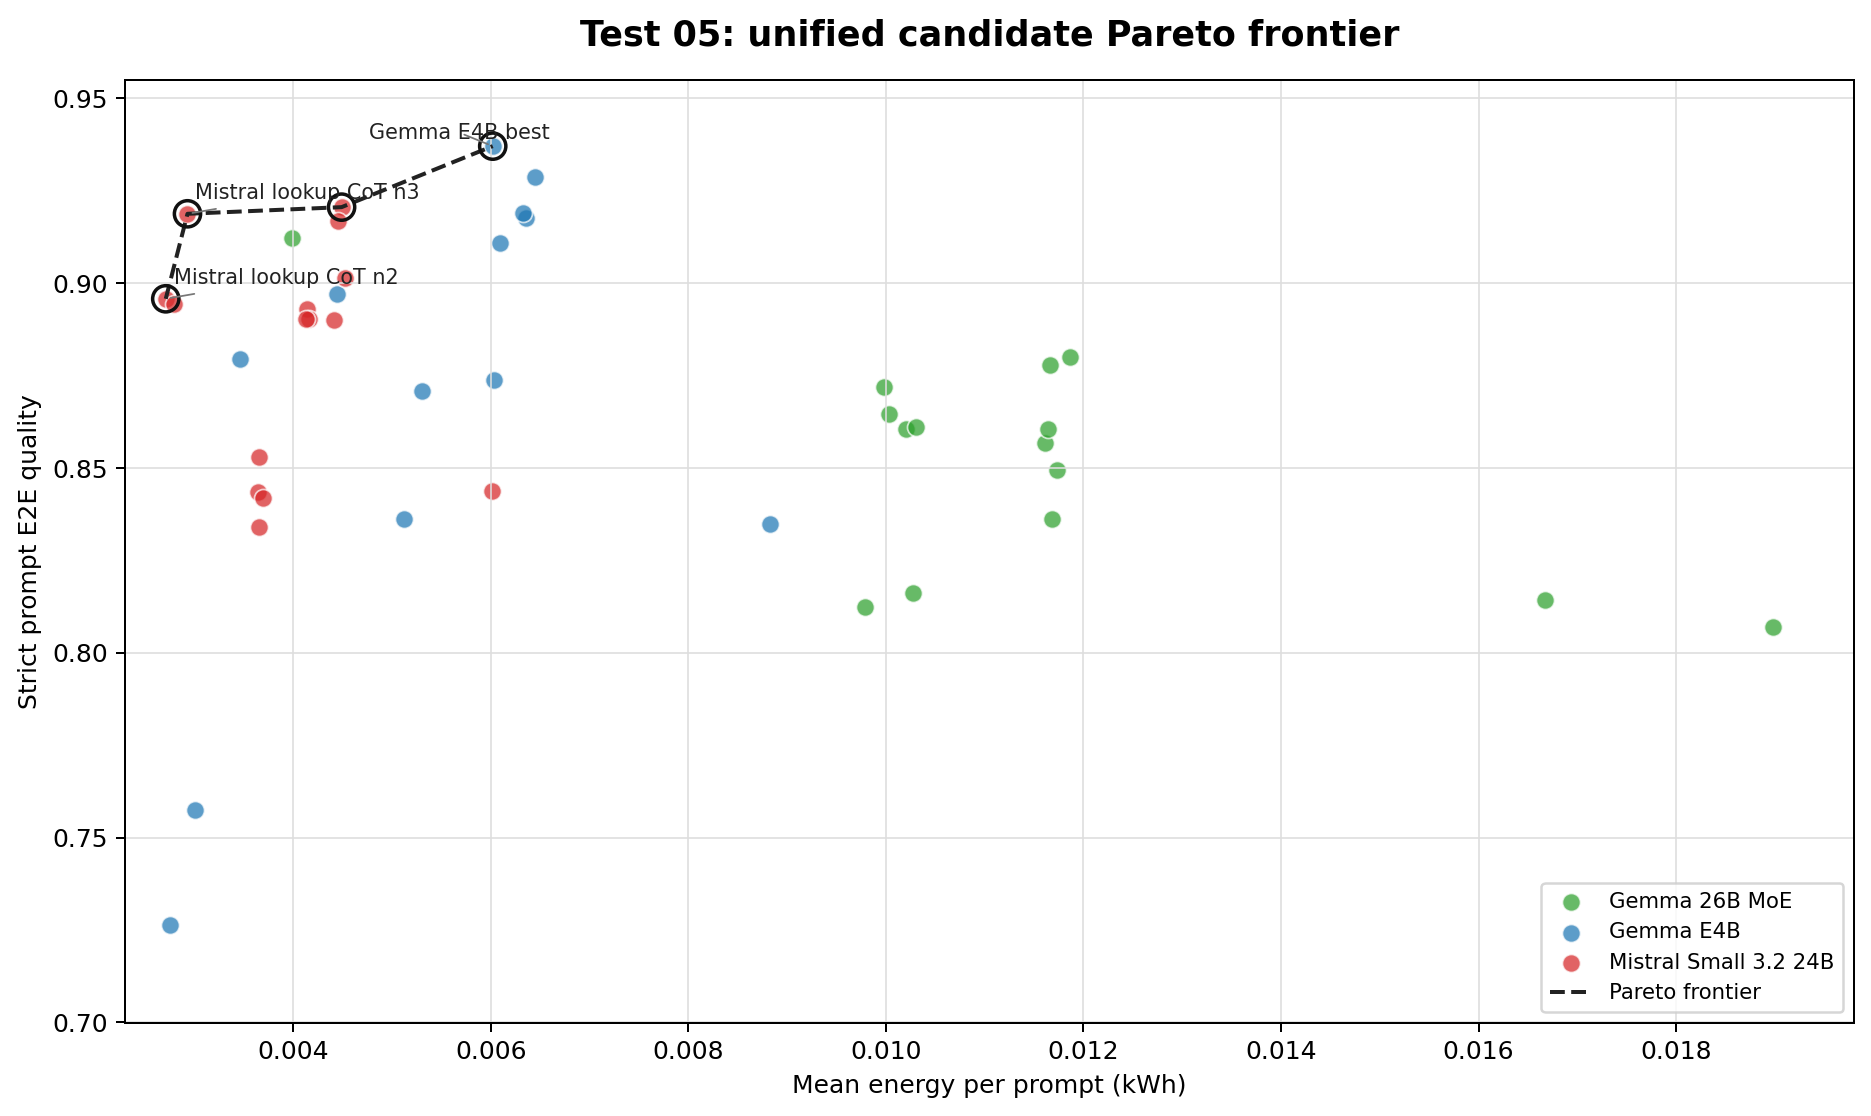
\includegraphics[width=\columnwidth]{Images/test05_final_run_unified_candidate_pareto.png}
    \caption{Test~05: unified quality--energy Pareto frontier among the evaluated candidate configurations.}
    \label{fig:es_pareto}
\end{figure}

%-----------------------------------------------------------------------------
% CONCLUSIONS
%-----------------------------------------------------------------------------
\section{Conclusions}
\label{sec:es_conclusions}

This work studied the quality--latency--energy trade-off of a multi-step LLM data agent for
sales analytics. The central result is that model choice alone does not explain performance:
the dominant effects emerge from the interaction between model family, agent step, prompt
difficulty, and inference-time parameters. The untuned baseline favours Mistral~Small for its
efficiency, but the difficulty split reveals what the aggregate hides --- it collapses on the
hardest SQL aggregations, exactly where targeted lookup repair lets the compact Gemma~E4B
compete with it. This repair comes specifically from CoT refinement, which exploits executable
SQL feedback; best-of-$N$ sampling, by contrast, was limited by the local selector, which
still preferred the first candidate in most Best-of-3 runs. After tuning, the
quality--energy frontier is defined by Mistral candidates, while Gemma~E4B remains a very
close high-quality alternative and the larger Gemma~26B improves yet stays dominated once
energy is counted. Notably, the recommended configurations improve substantially over their
untuned baselines, so per-step tuning is a genuine improvement rather than a simple
quality-for-energy trade.

From this evidence the thesis distils three practical recommendations for energy-aware LLM
data agents:

\begin{enumerate}[noitemsep,topsep=2pt]
    \item \textbf{Tune per agent step, not globally.} Sensitivity is a model-level property,
          and the most rewarding target and safe operating range differ by step, so a single
          global setting leaves quality on the table.
    \item \textbf{Allocate inference-time compute by failure mode.} Grant token headroom only
          to genuinely truncated steps, apply CoT refinement where feedback is verifiable
          (SQL lookup), and keep generation conservative where errors are semantic
          (visualization).
    \item \textbf{Report accuracy and energy by prompt difficulty,} since the best model for
          simple tasks is not the best for hard analytical questions.
\end{enumerate}


%---------------------------------------------------------------------------
%  BIBLIOGRAPHY
%---------------------------------------------------------------------------
% Remember to insert here only the essential bibliography of your work
\bibliography{bibliography.bib} % automatically inserted and ordered with this command

\end{document}
